\begin{figure}[!b]
  \centering
    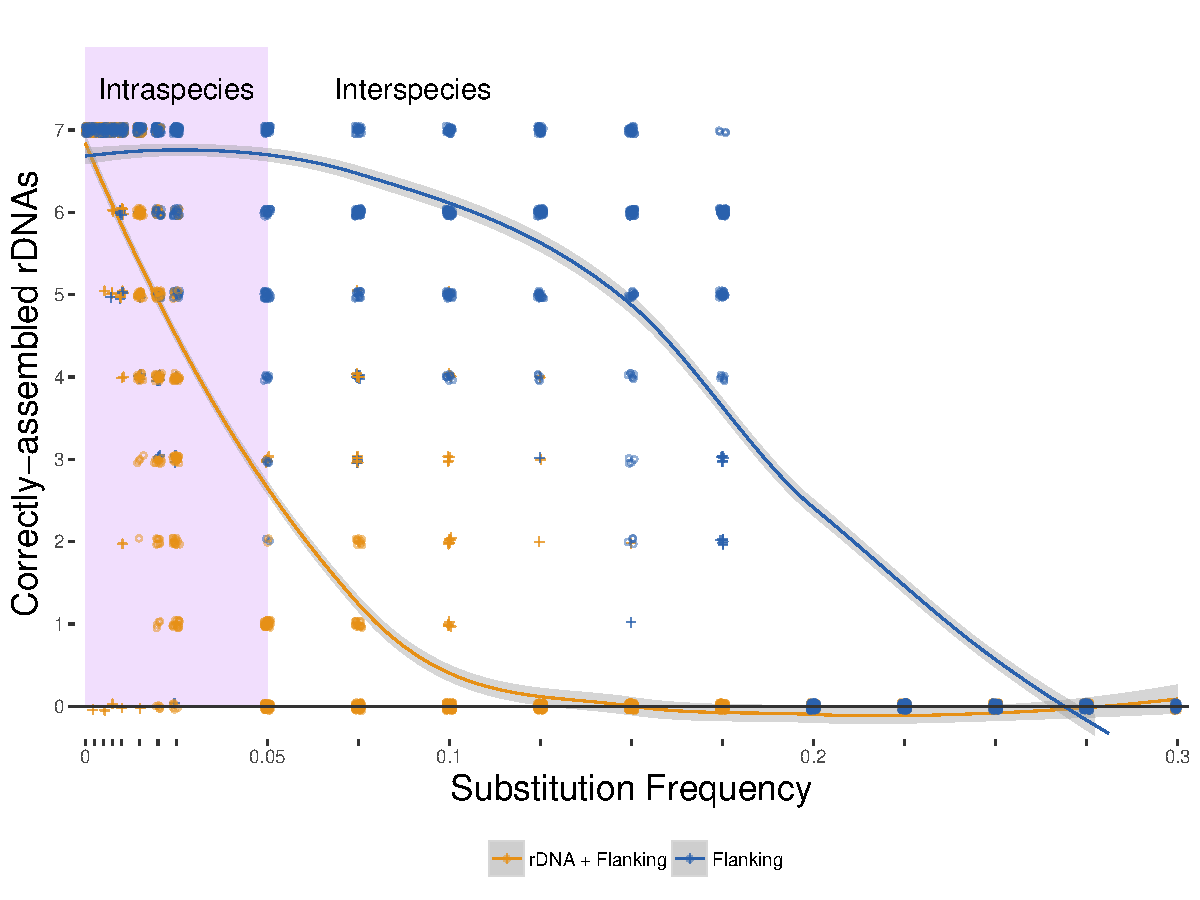
\includegraphics[width=.9\columnwidth]{degenerate_lineplot}
  \caption{Variants of the artificial chromosome with substitution frequencies between 0 and 0.3 (i.e. up to 300 substitutions per kb). Correctly-assembled rDNAs were counted, and the distribution of results shown against the appropriate substitution frequency. Results are shown for models where substitutions are permitted throughout the chromosome (orange), and only in the flanking regions (blue), the latter approximating the relative rate of substitution in rDNA and flanking regions. Lilac area corresponds to substitution frequencies resulting in average sequence identity over 95\%, denoting an estimated species boundary. Loess smoothing was used to generate the blue and yellow trendlines. Outliers are shown as $+$'s. n=100.}
  \label{fig:degen}
\end{figure}
